
% Default to the notebook output style

    


% Inherit from the specified cell style.




    
\documentclass[11pt]{article}

    
    
    \usepackage[T1]{fontenc}
    % Nicer default font (+ math font) than Computer Modern for most use cases
    \usepackage{mathpazo}

    % Basic figure setup, for now with no caption control since it's done
    % automatically by Pandoc (which extracts ![](path) syntax from Markdown).
    \usepackage{graphicx}
    % We will generate all images so they have a width \maxwidth. This means
    % that they will get their normal width if they fit onto the page, but
    % are scaled down if they would overflow the margins.
    \makeatletter
    \def\maxwidth{\ifdim\Gin@nat@width>\linewidth\linewidth
    \else\Gin@nat@width\fi}
    \makeatother
    \let\Oldincludegraphics\includegraphics
    % Set max figure width to be 80% of text width, for now hardcoded.
    \renewcommand{\includegraphics}[1]{\Oldincludegraphics[width=.8\maxwidth]{#1}}
    % Ensure that by default, figures have no caption (until we provide a
    % proper Figure object with a Caption API and a way to capture that
    % in the conversion process - todo).
    \usepackage{caption}
    \DeclareCaptionLabelFormat{nolabel}{}
    \captionsetup{labelformat=nolabel}

    \usepackage{adjustbox} % Used to constrain images to a maximum size 
    \usepackage{xcolor} % Allow colors to be defined
    \usepackage{enumerate} % Needed for markdown enumerations to work
    \usepackage{geometry} % Used to adjust the document margins
    \usepackage{amsmath} % Equations
    \usepackage{amssymb} % Equations
    \usepackage{textcomp} % defines textquotesingle
    % Hack from http://tex.stackexchange.com/a/47451/13684:
    \AtBeginDocument{%
        \def\PYZsq{\textquotesingle}% Upright quotes in Pygmentized code
    }
    \usepackage{upquote} % Upright quotes for verbatim code
    \usepackage{eurosym} % defines \euro
    \usepackage[mathletters]{ucs} % Extended unicode (utf-8) support
    \usepackage[utf8x]{inputenc} % Allow utf-8 characters in the tex document
    \usepackage{fancyvrb} % verbatim replacement that allows latex
    \usepackage{grffile} % extends the file name processing of package graphics 
                         % to support a larger range 
    % The hyperref package gives us a pdf with properly built
    % internal navigation ('pdf bookmarks' for the table of contents,
    % internal cross-reference links, web links for URLs, etc.)
    \usepackage{hyperref}
    \usepackage{longtable} % longtable support required by pandoc >1.10
    \usepackage{booktabs}  % table support for pandoc > 1.12.2
    \usepackage[inline]{enumitem} % IRkernel/repr support (it uses the enumerate* environment)
    \usepackage[normalem]{ulem} % ulem is needed to support strikethroughs (\sout)
                                % normalem makes italics be italics, not underlines
    

    
    
    % Colors for the hyperref package
    \definecolor{urlcolor}{rgb}{0,.145,.698}
    \definecolor{linkcolor}{rgb}{.71,0.21,0.01}
    \definecolor{citecolor}{rgb}{.12,.54,.11}

    % ANSI colors
    \definecolor{ansi-black}{HTML}{3E424D}
    \definecolor{ansi-black-intense}{HTML}{282C36}
    \definecolor{ansi-red}{HTML}{E75C58}
    \definecolor{ansi-red-intense}{HTML}{B22B31}
    \definecolor{ansi-green}{HTML}{00A250}
    \definecolor{ansi-green-intense}{HTML}{007427}
    \definecolor{ansi-yellow}{HTML}{DDB62B}
    \definecolor{ansi-yellow-intense}{HTML}{B27D12}
    \definecolor{ansi-blue}{HTML}{208FFB}
    \definecolor{ansi-blue-intense}{HTML}{0065CA}
    \definecolor{ansi-magenta}{HTML}{D160C4}
    \definecolor{ansi-magenta-intense}{HTML}{A03196}
    \definecolor{ansi-cyan}{HTML}{60C6C8}
    \definecolor{ansi-cyan-intense}{HTML}{258F8F}
    \definecolor{ansi-white}{HTML}{C5C1B4}
    \definecolor{ansi-white-intense}{HTML}{A1A6B2}

    % commands and environments needed by pandoc snippets
    % extracted from the output of `pandoc -s`
    \providecommand{\tightlist}{%
      \setlength{\itemsep}{0pt}\setlength{\parskip}{0pt}}
    \DefineVerbatimEnvironment{Highlighting}{Verbatim}{commandchars=\\\{\}}
    % Add ',fontsize=\small' for more characters per line
    \newenvironment{Shaded}{}{}
    \newcommand{\KeywordTok}[1]{\textcolor[rgb]{0.00,0.44,0.13}{\textbf{{#1}}}}
    \newcommand{\DataTypeTok}[1]{\textcolor[rgb]{0.56,0.13,0.00}{{#1}}}
    \newcommand{\DecValTok}[1]{\textcolor[rgb]{0.25,0.63,0.44}{{#1}}}
    \newcommand{\BaseNTok}[1]{\textcolor[rgb]{0.25,0.63,0.44}{{#1}}}
    \newcommand{\FloatTok}[1]{\textcolor[rgb]{0.25,0.63,0.44}{{#1}}}
    \newcommand{\CharTok}[1]{\textcolor[rgb]{0.25,0.44,0.63}{{#1}}}
    \newcommand{\StringTok}[1]{\textcolor[rgb]{0.25,0.44,0.63}{{#1}}}
    \newcommand{\CommentTok}[1]{\textcolor[rgb]{0.38,0.63,0.69}{\textit{{#1}}}}
    \newcommand{\OtherTok}[1]{\textcolor[rgb]{0.00,0.44,0.13}{{#1}}}
    \newcommand{\AlertTok}[1]{\textcolor[rgb]{1.00,0.00,0.00}{\textbf{{#1}}}}
    \newcommand{\FunctionTok}[1]{\textcolor[rgb]{0.02,0.16,0.49}{{#1}}}
    \newcommand{\RegionMarkerTok}[1]{{#1}}
    \newcommand{\ErrorTok}[1]{\textcolor[rgb]{1.00,0.00,0.00}{\textbf{{#1}}}}
    \newcommand{\NormalTok}[1]{{#1}}
    
    % Additional commands for more recent versions of Pandoc
    \newcommand{\ConstantTok}[1]{\textcolor[rgb]{0.53,0.00,0.00}{{#1}}}
    \newcommand{\SpecialCharTok}[1]{\textcolor[rgb]{0.25,0.44,0.63}{{#1}}}
    \newcommand{\VerbatimStringTok}[1]{\textcolor[rgb]{0.25,0.44,0.63}{{#1}}}
    \newcommand{\SpecialStringTok}[1]{\textcolor[rgb]{0.73,0.40,0.53}{{#1}}}
    \newcommand{\ImportTok}[1]{{#1}}
    \newcommand{\DocumentationTok}[1]{\textcolor[rgb]{0.73,0.13,0.13}{\textit{{#1}}}}
    \newcommand{\AnnotationTok}[1]{\textcolor[rgb]{0.38,0.63,0.69}{\textbf{\textit{{#1}}}}}
    \newcommand{\CommentVarTok}[1]{\textcolor[rgb]{0.38,0.63,0.69}{\textbf{\textit{{#1}}}}}
    \newcommand{\VariableTok}[1]{\textcolor[rgb]{0.10,0.09,0.49}{{#1}}}
    \newcommand{\ControlFlowTok}[1]{\textcolor[rgb]{0.00,0.44,0.13}{\textbf{{#1}}}}
    \newcommand{\OperatorTok}[1]{\textcolor[rgb]{0.40,0.40,0.40}{{#1}}}
    \newcommand{\BuiltInTok}[1]{{#1}}
    \newcommand{\ExtensionTok}[1]{{#1}}
    \newcommand{\PreprocessorTok}[1]{\textcolor[rgb]{0.74,0.48,0.00}{{#1}}}
    \newcommand{\AttributeTok}[1]{\textcolor[rgb]{0.49,0.56,0.16}{{#1}}}
    \newcommand{\InformationTok}[1]{\textcolor[rgb]{0.38,0.63,0.69}{\textbf{\textit{{#1}}}}}
    \newcommand{\WarningTok}[1]{\textcolor[rgb]{0.38,0.63,0.69}{\textbf{\textit{{#1}}}}}
    
    
    % Define a nice break command that doesn't care if a line doesn't already
    % exist.
    \def\br{\hspace*{\fill} \\* }
    % Math Jax compatability definitions
    \def\gt{>}
    \def\lt{<}
    % Document parameters
    \title{RoomCoulingFV}
    
    
    

    % Pygments definitions
    
\makeatletter
\def\PY@reset{\let\PY@it=\relax \let\PY@bf=\relax%
    \let\PY@ul=\relax \let\PY@tc=\relax%
    \let\PY@bc=\relax \let\PY@ff=\relax}
\def\PY@tok#1{\csname PY@tok@#1\endcsname}
\def\PY@toks#1+{\ifx\relax#1\empty\else%
    \PY@tok{#1}\expandafter\PY@toks\fi}
\def\PY@do#1{\PY@bc{\PY@tc{\PY@ul{%
    \PY@it{\PY@bf{\PY@ff{#1}}}}}}}
\def\PY#1#2{\PY@reset\PY@toks#1+\relax+\PY@do{#2}}

\expandafter\def\csname PY@tok@w\endcsname{\def\PY@tc##1{\textcolor[rgb]{0.73,0.73,0.73}{##1}}}
\expandafter\def\csname PY@tok@c\endcsname{\let\PY@it=\textit\def\PY@tc##1{\textcolor[rgb]{0.25,0.50,0.50}{##1}}}
\expandafter\def\csname PY@tok@cp\endcsname{\def\PY@tc##1{\textcolor[rgb]{0.74,0.48,0.00}{##1}}}
\expandafter\def\csname PY@tok@k\endcsname{\let\PY@bf=\textbf\def\PY@tc##1{\textcolor[rgb]{0.00,0.50,0.00}{##1}}}
\expandafter\def\csname PY@tok@kp\endcsname{\def\PY@tc##1{\textcolor[rgb]{0.00,0.50,0.00}{##1}}}
\expandafter\def\csname PY@tok@kt\endcsname{\def\PY@tc##1{\textcolor[rgb]{0.69,0.00,0.25}{##1}}}
\expandafter\def\csname PY@tok@o\endcsname{\def\PY@tc##1{\textcolor[rgb]{0.40,0.40,0.40}{##1}}}
\expandafter\def\csname PY@tok@ow\endcsname{\let\PY@bf=\textbf\def\PY@tc##1{\textcolor[rgb]{0.67,0.13,1.00}{##1}}}
\expandafter\def\csname PY@tok@nb\endcsname{\def\PY@tc##1{\textcolor[rgb]{0.00,0.50,0.00}{##1}}}
\expandafter\def\csname PY@tok@nf\endcsname{\def\PY@tc##1{\textcolor[rgb]{0.00,0.00,1.00}{##1}}}
\expandafter\def\csname PY@tok@nc\endcsname{\let\PY@bf=\textbf\def\PY@tc##1{\textcolor[rgb]{0.00,0.00,1.00}{##1}}}
\expandafter\def\csname PY@tok@nn\endcsname{\let\PY@bf=\textbf\def\PY@tc##1{\textcolor[rgb]{0.00,0.00,1.00}{##1}}}
\expandafter\def\csname PY@tok@ne\endcsname{\let\PY@bf=\textbf\def\PY@tc##1{\textcolor[rgb]{0.82,0.25,0.23}{##1}}}
\expandafter\def\csname PY@tok@nv\endcsname{\def\PY@tc##1{\textcolor[rgb]{0.10,0.09,0.49}{##1}}}
\expandafter\def\csname PY@tok@no\endcsname{\def\PY@tc##1{\textcolor[rgb]{0.53,0.00,0.00}{##1}}}
\expandafter\def\csname PY@tok@nl\endcsname{\def\PY@tc##1{\textcolor[rgb]{0.63,0.63,0.00}{##1}}}
\expandafter\def\csname PY@tok@ni\endcsname{\let\PY@bf=\textbf\def\PY@tc##1{\textcolor[rgb]{0.60,0.60,0.60}{##1}}}
\expandafter\def\csname PY@tok@na\endcsname{\def\PY@tc##1{\textcolor[rgb]{0.49,0.56,0.16}{##1}}}
\expandafter\def\csname PY@tok@nt\endcsname{\let\PY@bf=\textbf\def\PY@tc##1{\textcolor[rgb]{0.00,0.50,0.00}{##1}}}
\expandafter\def\csname PY@tok@nd\endcsname{\def\PY@tc##1{\textcolor[rgb]{0.67,0.13,1.00}{##1}}}
\expandafter\def\csname PY@tok@s\endcsname{\def\PY@tc##1{\textcolor[rgb]{0.73,0.13,0.13}{##1}}}
\expandafter\def\csname PY@tok@sd\endcsname{\let\PY@it=\textit\def\PY@tc##1{\textcolor[rgb]{0.73,0.13,0.13}{##1}}}
\expandafter\def\csname PY@tok@si\endcsname{\let\PY@bf=\textbf\def\PY@tc##1{\textcolor[rgb]{0.73,0.40,0.53}{##1}}}
\expandafter\def\csname PY@tok@se\endcsname{\let\PY@bf=\textbf\def\PY@tc##1{\textcolor[rgb]{0.73,0.40,0.13}{##1}}}
\expandafter\def\csname PY@tok@sr\endcsname{\def\PY@tc##1{\textcolor[rgb]{0.73,0.40,0.53}{##1}}}
\expandafter\def\csname PY@tok@ss\endcsname{\def\PY@tc##1{\textcolor[rgb]{0.10,0.09,0.49}{##1}}}
\expandafter\def\csname PY@tok@sx\endcsname{\def\PY@tc##1{\textcolor[rgb]{0.00,0.50,0.00}{##1}}}
\expandafter\def\csname PY@tok@m\endcsname{\def\PY@tc##1{\textcolor[rgb]{0.40,0.40,0.40}{##1}}}
\expandafter\def\csname PY@tok@gh\endcsname{\let\PY@bf=\textbf\def\PY@tc##1{\textcolor[rgb]{0.00,0.00,0.50}{##1}}}
\expandafter\def\csname PY@tok@gu\endcsname{\let\PY@bf=\textbf\def\PY@tc##1{\textcolor[rgb]{0.50,0.00,0.50}{##1}}}
\expandafter\def\csname PY@tok@gd\endcsname{\def\PY@tc##1{\textcolor[rgb]{0.63,0.00,0.00}{##1}}}
\expandafter\def\csname PY@tok@gi\endcsname{\def\PY@tc##1{\textcolor[rgb]{0.00,0.63,0.00}{##1}}}
\expandafter\def\csname PY@tok@gr\endcsname{\def\PY@tc##1{\textcolor[rgb]{1.00,0.00,0.00}{##1}}}
\expandafter\def\csname PY@tok@ge\endcsname{\let\PY@it=\textit}
\expandafter\def\csname PY@tok@gs\endcsname{\let\PY@bf=\textbf}
\expandafter\def\csname PY@tok@gp\endcsname{\let\PY@bf=\textbf\def\PY@tc##1{\textcolor[rgb]{0.00,0.00,0.50}{##1}}}
\expandafter\def\csname PY@tok@go\endcsname{\def\PY@tc##1{\textcolor[rgb]{0.53,0.53,0.53}{##1}}}
\expandafter\def\csname PY@tok@gt\endcsname{\def\PY@tc##1{\textcolor[rgb]{0.00,0.27,0.87}{##1}}}
\expandafter\def\csname PY@tok@err\endcsname{\def\PY@bc##1{\setlength{\fboxsep}{0pt}\fcolorbox[rgb]{1.00,0.00,0.00}{1,1,1}{\strut ##1}}}
\expandafter\def\csname PY@tok@kc\endcsname{\let\PY@bf=\textbf\def\PY@tc##1{\textcolor[rgb]{0.00,0.50,0.00}{##1}}}
\expandafter\def\csname PY@tok@kd\endcsname{\let\PY@bf=\textbf\def\PY@tc##1{\textcolor[rgb]{0.00,0.50,0.00}{##1}}}
\expandafter\def\csname PY@tok@kn\endcsname{\let\PY@bf=\textbf\def\PY@tc##1{\textcolor[rgb]{0.00,0.50,0.00}{##1}}}
\expandafter\def\csname PY@tok@kr\endcsname{\let\PY@bf=\textbf\def\PY@tc##1{\textcolor[rgb]{0.00,0.50,0.00}{##1}}}
\expandafter\def\csname PY@tok@bp\endcsname{\def\PY@tc##1{\textcolor[rgb]{0.00,0.50,0.00}{##1}}}
\expandafter\def\csname PY@tok@fm\endcsname{\def\PY@tc##1{\textcolor[rgb]{0.00,0.00,1.00}{##1}}}
\expandafter\def\csname PY@tok@vc\endcsname{\def\PY@tc##1{\textcolor[rgb]{0.10,0.09,0.49}{##1}}}
\expandafter\def\csname PY@tok@vg\endcsname{\def\PY@tc##1{\textcolor[rgb]{0.10,0.09,0.49}{##1}}}
\expandafter\def\csname PY@tok@vi\endcsname{\def\PY@tc##1{\textcolor[rgb]{0.10,0.09,0.49}{##1}}}
\expandafter\def\csname PY@tok@vm\endcsname{\def\PY@tc##1{\textcolor[rgb]{0.10,0.09,0.49}{##1}}}
\expandafter\def\csname PY@tok@sa\endcsname{\def\PY@tc##1{\textcolor[rgb]{0.73,0.13,0.13}{##1}}}
\expandafter\def\csname PY@tok@sb\endcsname{\def\PY@tc##1{\textcolor[rgb]{0.73,0.13,0.13}{##1}}}
\expandafter\def\csname PY@tok@sc\endcsname{\def\PY@tc##1{\textcolor[rgb]{0.73,0.13,0.13}{##1}}}
\expandafter\def\csname PY@tok@dl\endcsname{\def\PY@tc##1{\textcolor[rgb]{0.73,0.13,0.13}{##1}}}
\expandafter\def\csname PY@tok@s2\endcsname{\def\PY@tc##1{\textcolor[rgb]{0.73,0.13,0.13}{##1}}}
\expandafter\def\csname PY@tok@sh\endcsname{\def\PY@tc##1{\textcolor[rgb]{0.73,0.13,0.13}{##1}}}
\expandafter\def\csname PY@tok@s1\endcsname{\def\PY@tc##1{\textcolor[rgb]{0.73,0.13,0.13}{##1}}}
\expandafter\def\csname PY@tok@mb\endcsname{\def\PY@tc##1{\textcolor[rgb]{0.40,0.40,0.40}{##1}}}
\expandafter\def\csname PY@tok@mf\endcsname{\def\PY@tc##1{\textcolor[rgb]{0.40,0.40,0.40}{##1}}}
\expandafter\def\csname PY@tok@mh\endcsname{\def\PY@tc##1{\textcolor[rgb]{0.40,0.40,0.40}{##1}}}
\expandafter\def\csname PY@tok@mi\endcsname{\def\PY@tc##1{\textcolor[rgb]{0.40,0.40,0.40}{##1}}}
\expandafter\def\csname PY@tok@il\endcsname{\def\PY@tc##1{\textcolor[rgb]{0.40,0.40,0.40}{##1}}}
\expandafter\def\csname PY@tok@mo\endcsname{\def\PY@tc##1{\textcolor[rgb]{0.40,0.40,0.40}{##1}}}
\expandafter\def\csname PY@tok@ch\endcsname{\let\PY@it=\textit\def\PY@tc##1{\textcolor[rgb]{0.25,0.50,0.50}{##1}}}
\expandafter\def\csname PY@tok@cm\endcsname{\let\PY@it=\textit\def\PY@tc##1{\textcolor[rgb]{0.25,0.50,0.50}{##1}}}
\expandafter\def\csname PY@tok@cpf\endcsname{\let\PY@it=\textit\def\PY@tc##1{\textcolor[rgb]{0.25,0.50,0.50}{##1}}}
\expandafter\def\csname PY@tok@c1\endcsname{\let\PY@it=\textit\def\PY@tc##1{\textcolor[rgb]{0.25,0.50,0.50}{##1}}}
\expandafter\def\csname PY@tok@cs\endcsname{\let\PY@it=\textit\def\PY@tc##1{\textcolor[rgb]{0.25,0.50,0.50}{##1}}}

\def\PYZbs{\char`\\}
\def\PYZus{\char`\_}
\def\PYZob{\char`\{}
\def\PYZcb{\char`\}}
\def\PYZca{\char`\^}
\def\PYZam{\char`\&}
\def\PYZlt{\char`\<}
\def\PYZgt{\char`\>}
\def\PYZsh{\char`\#}
\def\PYZpc{\char`\%}
\def\PYZdl{\char`\$}
\def\PYZhy{\char`\-}
\def\PYZsq{\char`\'}
\def\PYZdq{\char`\"}
\def\PYZti{\char`\~}
% for compatibility with earlier versions
\def\PYZat{@}
\def\PYZlb{[}
\def\PYZrb{]}
\makeatother


    % Exact colors from NB
    \definecolor{incolor}{rgb}{0.0, 0.0, 0.5}
    \definecolor{outcolor}{rgb}{0.545, 0.0, 0.0}



    
    % Prevent overflowing lines due to hard-to-break entities
    \sloppy 
    % Setup hyperref package
    \hypersetup{
      breaklinks=true,  % so long urls are correctly broken across lines
      colorlinks=true,
      urlcolor=urlcolor,
      linkcolor=linkcolor,
      citecolor=citecolor,
      }
    % Slightly bigger margins than the latex defaults
    
    \geometry{verbose,tmargin=1in,bmargin=1in,lmargin=1in,rmargin=1in}
    
    

    \begin{document}
    
    
    \maketitle
    
    

    
    \hypertarget{stationary-heat-diffusion-problem-in-a-room-with-radiator-and-window}{%
\section{Stationary heat diffusion problem in a room with radiator and
window}\label{stationary-heat-diffusion-problem-in-a-room-with-radiator-and-window}}

\hypertarget{use-of-finite-volume-method}{%
\subsection{~ ~ ~ Use of finite volume
method}\label{use-of-finite-volume-method}}

\hypertarget{by-suxe9drick-kameni-ngwamou-phd-student.}{%
\subsection{~ ~ ~ (by Sédrick Kameni Ngwamou, PhD
student).}\label{by-suxe9drick-kameni-ngwamou-phd-student.}}

~ ~ The goal of this work is to determine the best position for a
radiator in a room with regard to the window position in order to
optimize the room temperature. The problem amounts to solving the
Laplace equation with Dirichlet boundary conditions in a cuboid
geometry. After meshing the room with tetrahedra or cubes, we use finite
volume method to compare three different radiator positions.\\
\hspace*{0.333em} ~ We start by recalling the existence theory for the
Laplace equation with smooth Dirichlet boundary conditions. We however
keep in mind that The application we have in mind has a discontinuous
boundary condition.

\hypertarget{variational-formulation-of-the-laplace-equation}{%
\subsection{1 - Variational formulation of the Laplace
equation}\label{variational-formulation-of-the-laplace-equation}}

Let \(d\in\mathbb{N}^*\) and \(\Omega\) a Lipschitz open subset of
\(\mathbb{R}^d\). Let \(g\in H^{\frac{1}{2}}(\partial\Omega)\) a
function defined on the boundary \(\partial\Omega\). We are interested
in the weak solutions of the following problem:

\[
\left\{\begin{array}{ccl}
-\triangle u=0 &\textrm{ in }& \Omega\\[1.5ex]
u=g &\textrm{ on } &\partial \Omega,    \;\;\;\;\;\;\;\;\;(1)    
       \end{array} 
\right.
\]

which means we are seeking for \(u\in H^1_g(\Omega)\) such that

\[
\forall v\in H^1_{g}(\Omega),\quad \int_\Omega \vec\nabla u\cdot\vec\nabla v - \int_{\partial\Omega}\vec\nabla u\cdot\vec n_x v\, d s_x = 0,\;\;\;\;\;\;\;\;\;(2)
\]

where \(H^1_g=\tilde g+H^1_0\) is the affine space

\[
H^1_g = \{u \in H^1(\Omega), u_{|\partial\Omega}=g\}
\]

with \(u_{|\partial\Omega}\) denoting the trace of \(u\) on
\(\partial\Omega\), and \(\tilde g\in H^1(\Omega)\) such that \(g\) is
the trace of \(\tilde g\) on \(\partial\Omega\).

\hypertarget{existence-of-the-solution}{%
\subsection{2 - Existence of the
solution}\label{existence-of-the-solution}}

Here we follow the method proposed by the remark 5.2.10 of {[}1{]} page
116. Using a change of variables, the boundary condition is set to
zeros. The problem comes down to solving the Poisson problem with a
source term in \(H^{-1}(\Omega)\).

\hypertarget{nonhomogeneous-problem}{%
\subsubsection{2.1 - Nonhomogeneous
problem}\label{nonhomogeneous-problem}}

Given that \(\Omega\) is Lipschitz, the trace operator is surjective
from \(H^{1}(\Omega)\) to \(H^{\frac{1}{2}}(\partial\Omega)\) (see
{[}1{]} remark 4.3.17, (or {[}2{]} remark 7-i) chapter 9 page 315 ).
Then there exists a function \(\tilde g\in H^{1}(\Omega)\) such that
\(\tilde g_{|\partial\Omega}=g\).

We want to prove the existence of the weak solution
\(\tilde u=u-\tilde g\in H^1_0(\Omega)\) of the following problem :

\[
\left\{\begin{array}{ccc}
-\triangle \tilde u=\triangle \tilde g &\textrm{ in }& \Omega\\[1.5ex]
\tilde u=0 &\textrm{ on } &\partial \Omega        
       \end{array}
\right.. \;\;\;\;\;\;\;\;\;(3)
\]

Given that \(\tilde g\in H^{1}(\Omega)\), we have
\(\triangle \tilde g \notin L^2(\Omega)\). In fact
\(\triangle \tilde g\) is not a function but a distribution:
\(\triangle \tilde g \in H^{-1}(\Omega)\), which does not prohibit the
use of the Lax-Milgram theorem.\\
As explained in the subsection 2.2 below, the Lax-Milgram theorem
implies the existence and uniqueness of \(\tilde u\in H^1_0(\Omega)\),
solution of (3). We deduce that \(u=\tilde u+\tilde g\in H^1_g\) is the
solution of (1).

\hypertarget{homogeneous-problem-with-fin-h-1}{%
\subsubsection{\texorpdfstring{2.2 - Homogeneous problem with
\(f\in H^{-1}\)}{2.2 - Homogeneous problem with f\textbackslash{}in H\^{}\{-1\}}}\label{homogeneous-problem-with-fin-h-1}}

We consider the following Poisson problem: find \(u\in H^1_0(\Omega)\)
weak solution of

\[
\left\{\begin{array}{ccc}
-\triangle u= f &\textrm{ in }& \Omega\\ 
u=0 &\textrm{ on } &\partial \Omega   \;\;\;\;\;\;\;\;\;(4)      
       \end{array}
\right.
\]

with \(f\in H^{-1}(\Omega)\). We recall that \(H^{-1}(\Omega)\) is the
set of linear continuous forms on \(H^{1}(\Omega)\). Elements of
\(H^{-1}(\Omega)\) are not functions but distributions, which does not
prohibit the use of the Lax-Milgram theorem.

In fact the variationnal formulation associated to (4) is

\[
\forall v\in H^1_0(\Omega),\quad \int_\Omega \vec\nabla u\cdot\vec\nabla v =\int_\Omega v\triangle g = - \int_{\Omega}\vec\nabla v\cdot\vec \nabla g.\;\;\;\;\;\;\;\;\;(5)
\]

The bilinear form \$ a( u,
v)=\int\emph{\Omega \vec\nabla u\cdot\vec\nabla v\$ is continuous and
coercive. The linear form \$ b(
v)=\int}\Omega \vec\nabla v\cdot\vec\nabla g\$ is continuous. The
Lax-Milgram theorem implies the existence of \(u\in H^1_0(\Omega)\) such
that \(a(u,v)=b(v) \: \forall v\in H^1_0(\Omega)\).

\hypertarget{the-two-point-finite-volume-scheme-for-the-stationary-diffusion-problem}{%
\subsection{3 - The two point finite volume scheme for the stationary
diffusion
problem}\label{the-two-point-finite-volume-scheme-for-the-stationary-diffusion-problem}}

The domain is decompose into cells \(K_i\): * \(|K_i|\) is the measure
of \(K_i\). * \(\sigma_{ij}\) the interface between two cells \(K_i\)
and \(K_j\). * \(|\sigma_{ij}|\) the measure of the interface
\(\sigma_{ij}\). * \(\vec{n}_{ij}\) the normal vector to the interface
between \(K_i\) and \(K_j\). * \(d_{ij}\) the distance between the
centers of mass of the two cells \(K_i\) and \(K_j\).

Then the discret problem is given by:

\[\left\{\begin{array}{ccl}
\sum\limits_{\sigma_{ij} \text{ interfaces of } K_i \text{ and } K_j} |\sigma_{ij}|F_{ij} = 0 &\textrm{ in }& \Omega\\[1.5ex]
u(x_b)=g &\textrm{ for } & x_b \in \partial \Omega,    \;\;\;\;\;\;\;\;\;(5)    
       \end{array}
\right.
\]

where \(F_{ij}\) is the numerical approximation of the outward normal
diffusion flux from the cell \(i\) to cell \(j\).

In the case of TPFA scheme, we have
\[F_{ij} = \frac{u_{K_i} - u_{K_j}}{d_{ij}}\vec{n}_{ij}\] for two
internal cells \(K_i\) and \(K_j\) and
\[F_{ib} = \frac{u_{K_i} - u(x_b)}{d_{ib}}\vec{n}_{ib}\] for the
boundary face with center \(x_b\), inner cell \(K_i\), outer normal
vector \(\vec{n}_{ib}\) and \(d_{ib}\) the distance between the center
of the cell \(K_i\) and \(x_b\).

\#\# 4 - Meshing and visualization of the results

In this section, We consider a room with a rectangular form with a
window at the middle of the back side. We then place the radiator in the
various position: * under the window, * on the side infront of the
window, * on the side at right of the window. The objective is to see
where is the good position we can place a radiator in a room in order to
have an optimal temperature in a room between certain range.

In this case we take \(\Omega =[0,4]\times[0,5]\times[0,3]\) and
\(\partial \Omega = \Gamma_1 \bigcup \Gamma_2\bigcup \Gamma_3\) such
that:

\[\Gamma_1 = Window\] \[\Gamma_2 = Radiator\] \[\Gamma_3 = Wall\]

To numerically solve this problem, we use the TPFA scheme in CoreFlows
library to carry out simulations.

we present de result obtain from a tetrahedral and a cubic meshes and
compare them.

    \hypertarget{shape}{%
\subsubsection{3.1 - shape}\label{shape}}

View of the back and right face\textbar{} View from the top without the
roof and the radiator in front -\textbar{} -
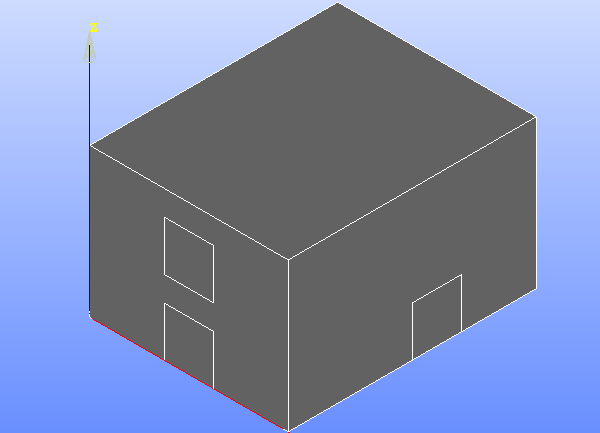
\includegraphics{SHView1.png}\textbar{} 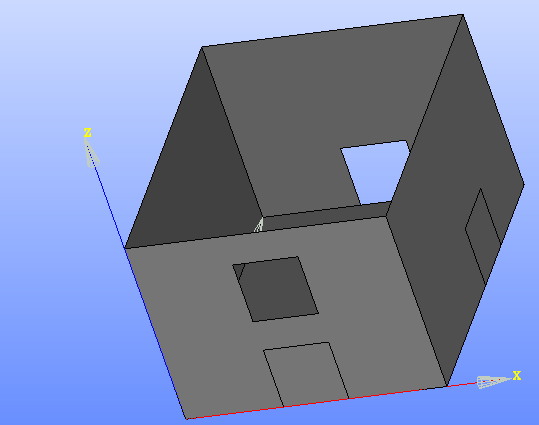
\includegraphics{SHNew2.png}

\hypertarget{meshes}{%
\subsubsection{3.2 - Meshes}\label{meshes}}

~ ~In this section we present meshes obtained by using mesh module of
Salome. At the left we have a 3D tetrahedra mesh which has been obtain
using the NETGEN 3D algorithm includ in in the mesh module. At the right
we have a cubic mesh obtained by combining the NETGEN 1D-2D algorithm
for the faces following by MG-HEXA algorithm for the 3D meshing. To be
able to manage the different boundary conditions (temperature on the
wall, window and radiator) given, we use the create group from geometry
option to create the different group (window, radiator and the wall).

\begin{longtable}[]{@{}ll@{}}
\toprule
Tetrahedral Mesh & Cubic mesh\tabularnewline
\midrule
\endhead
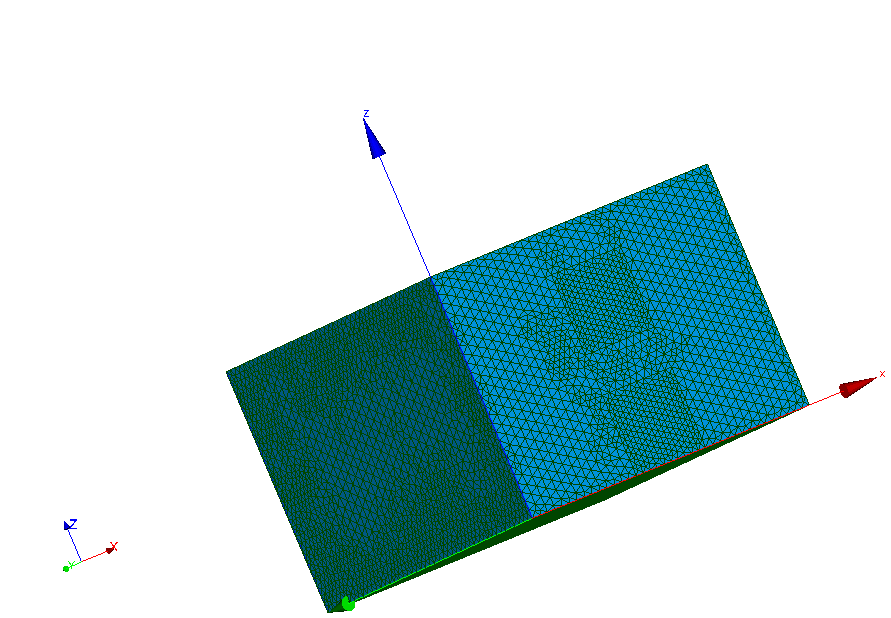
\includegraphics{Tetra147655.png} &
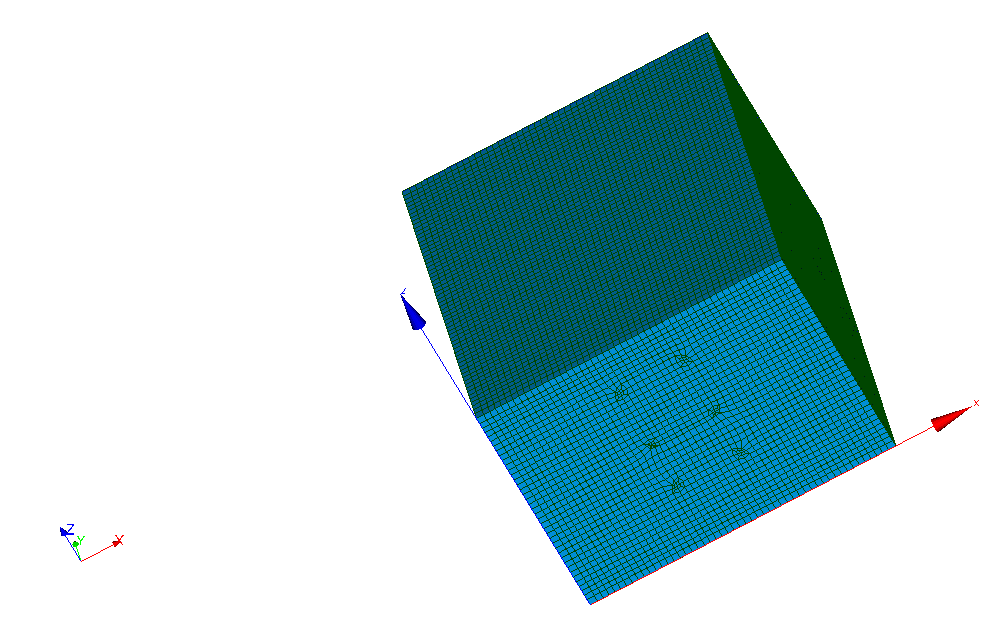
\includegraphics{MeshCubes140745.png}\tabularnewline
147 655 Cells & 140 745 Cells\tabularnewline
\bottomrule
\end{longtable}

    \hypertarget{visualization}{%
\subsubsection{3.3 - Visualization}\label{visualization}}

~ ~We consider that the temperature on the walls is \(20^\circ C\), the
radiator produces \(40^\circ C\) and temperature coming form the window
is \(0^\circ C\). We firstly present the result obtain with an
hexahedral meshing and then follows by the one with with cubic meshing.

\hypertarget{result-with-tetrahedral-mesh}{%
\paragraph{Result with tetrahedral
mesh}\label{result-with-tetrahedral-mesh}}

Radiator under window\textbar{} Radiator on the right wall \textbar{}
Radiator in the wall in front of the window - \textbar{} - -\textbar{}-
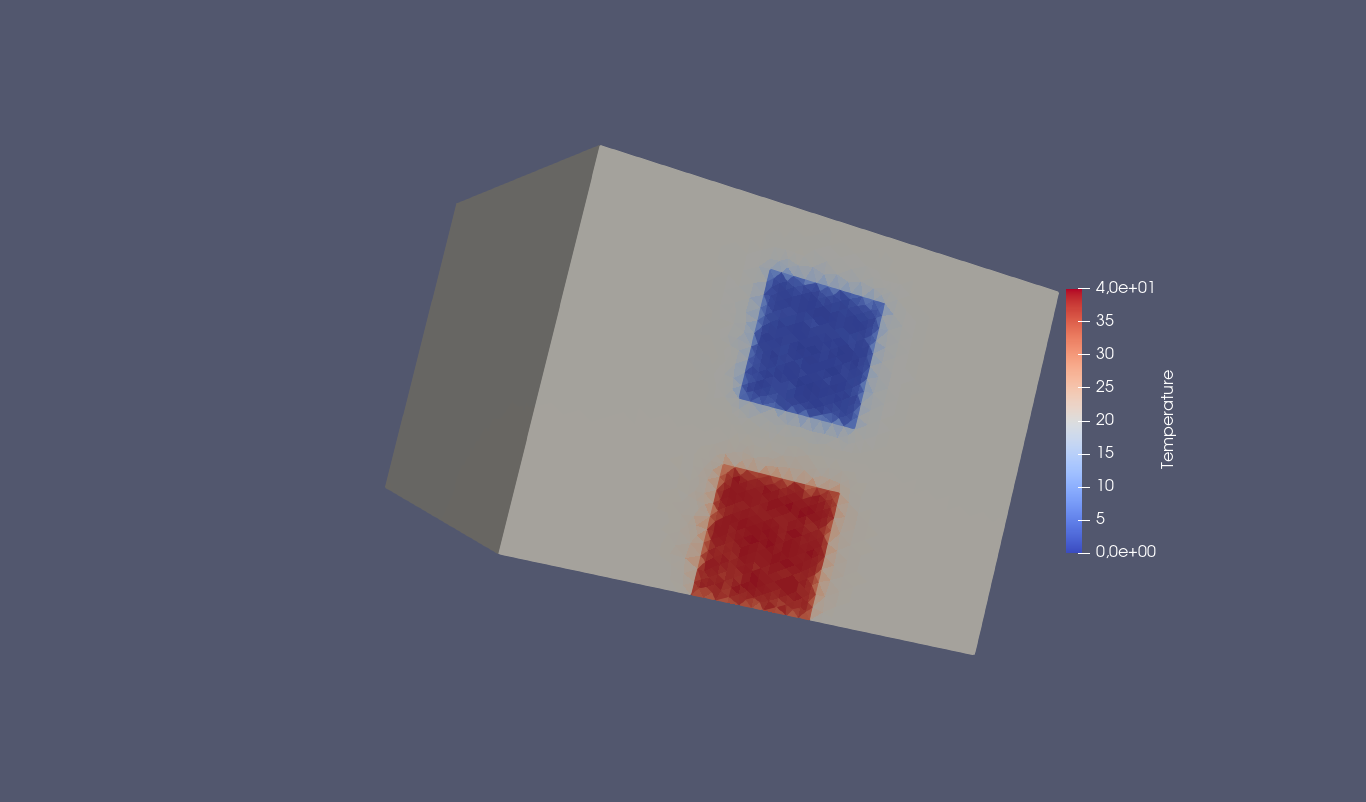
\includegraphics{FVTetra147655.png} \textbar{}
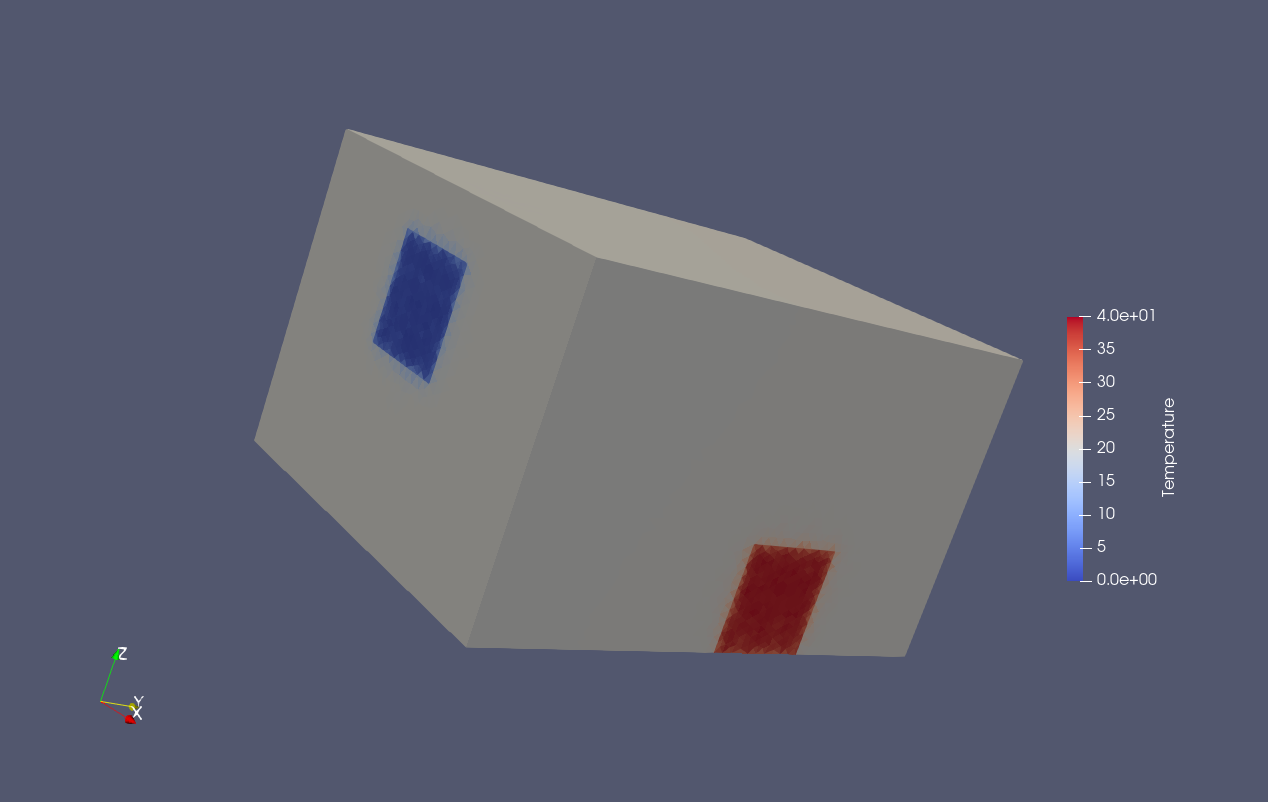
\includegraphics{ResultDroiteTetra.png} \textbar{}
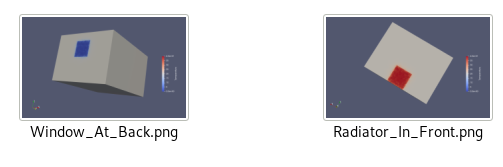
\includegraphics{TetraDevant.png}
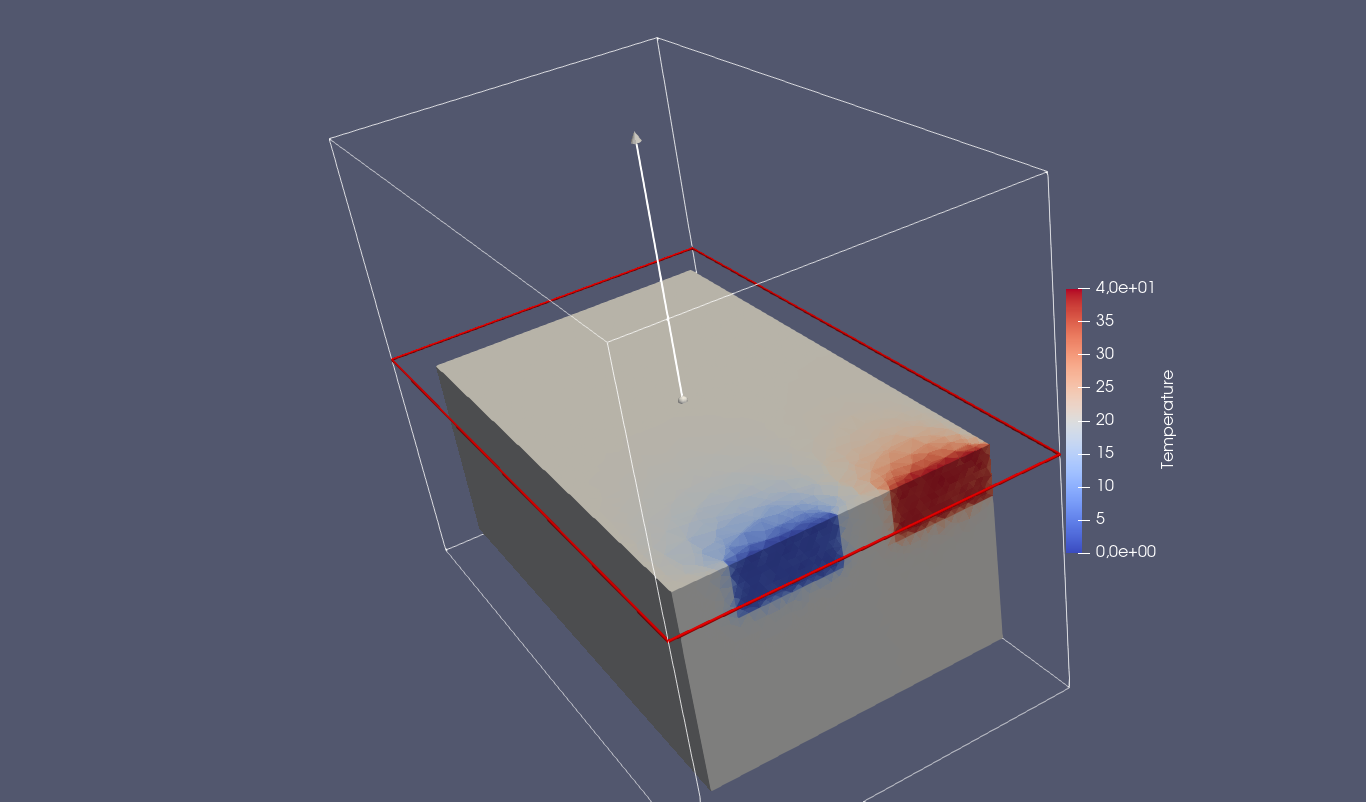
\includegraphics{ClipFVTetra147655.png} \textbar{}
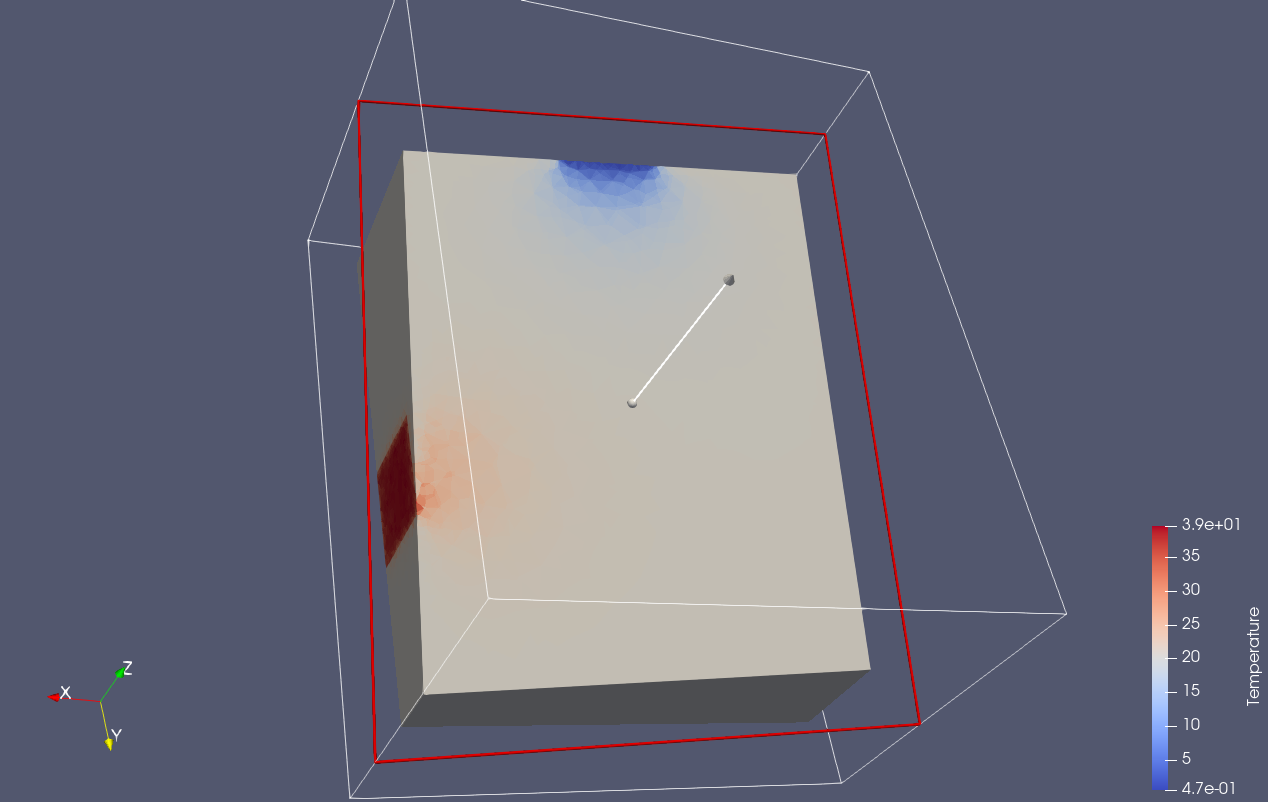
\includegraphics{ClipDroitTetra.png} \textbar{}
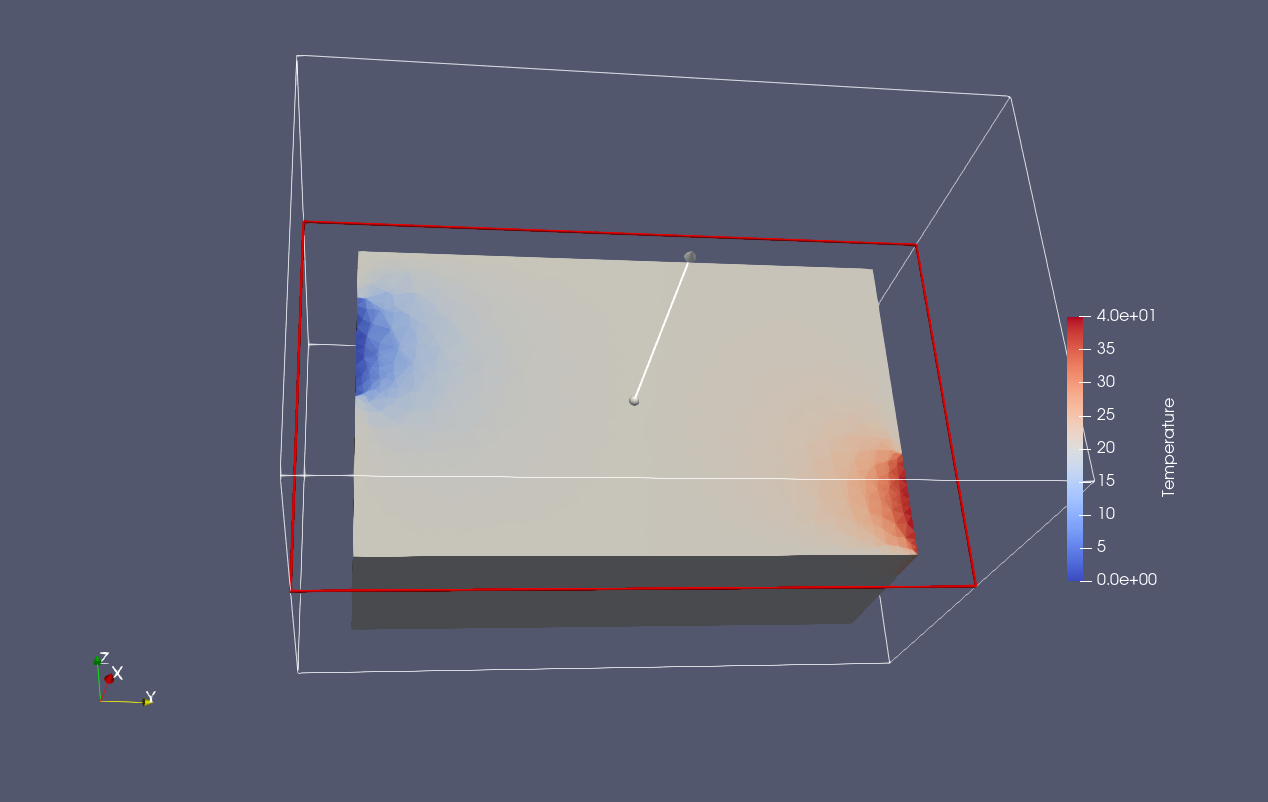
\includegraphics{ClipDevantTetra.png}

\hypertarget{result-with-cubic-mesh}{%
\paragraph{Result with cubic mesh}\label{result-with-cubic-mesh}}

Radiator under window\textbar{} Radiator on the right wall \textbar{}
Radiator in the wall in front of the window - \textbar{} - -\textbar{}-
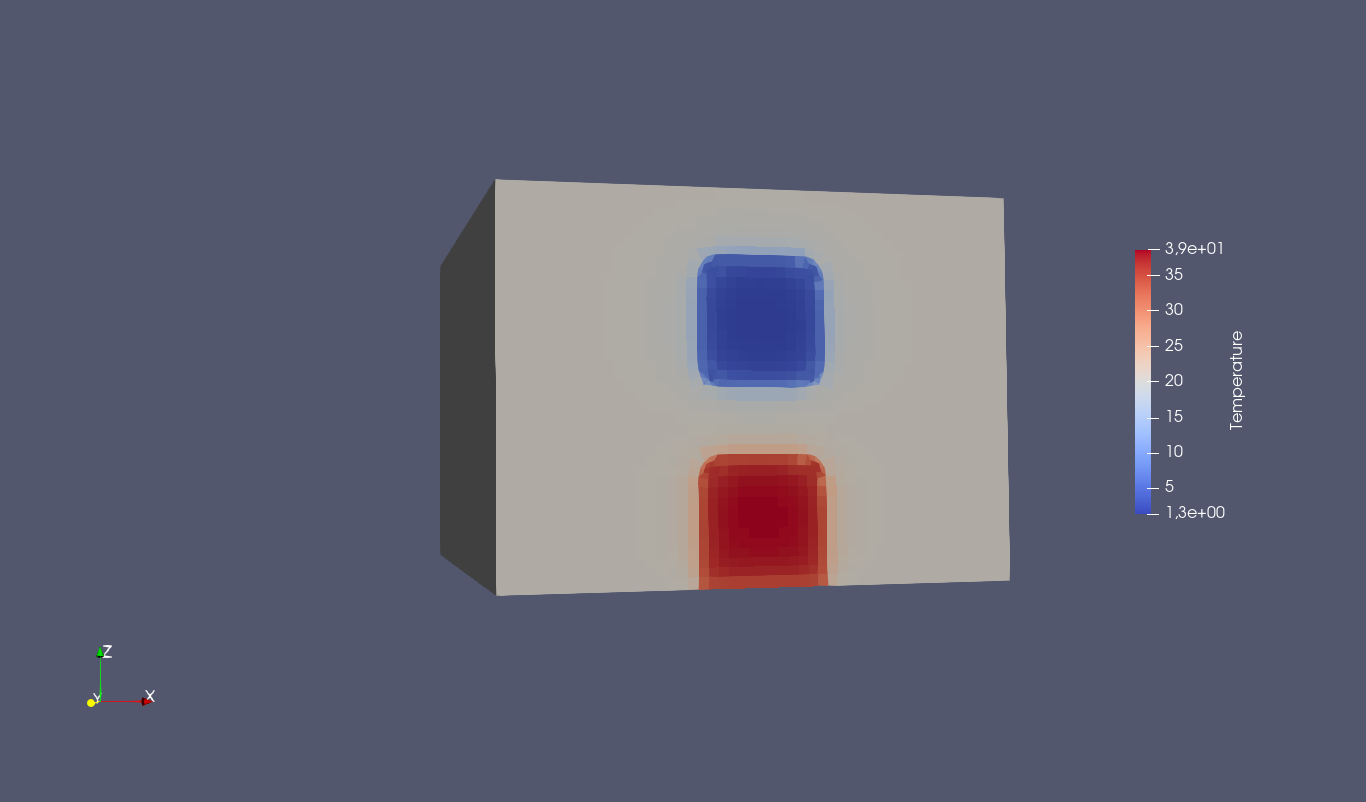
\includegraphics{RoomCouling140745.png} \textbar{}
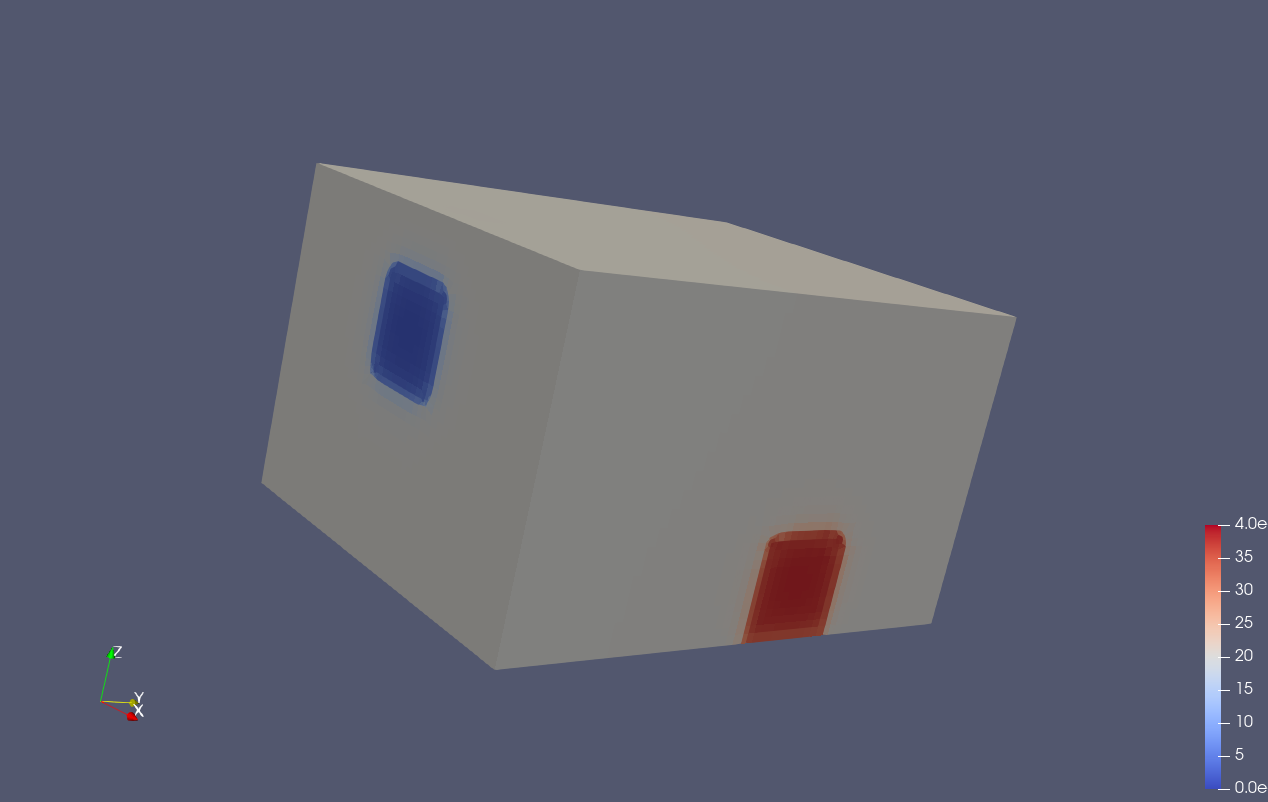
\includegraphics{ResutlDroitCubs.png} \textbar{}
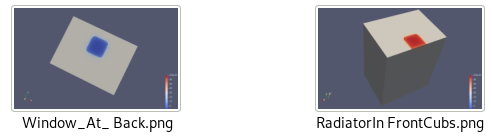
\includegraphics{CubesDevant.png} 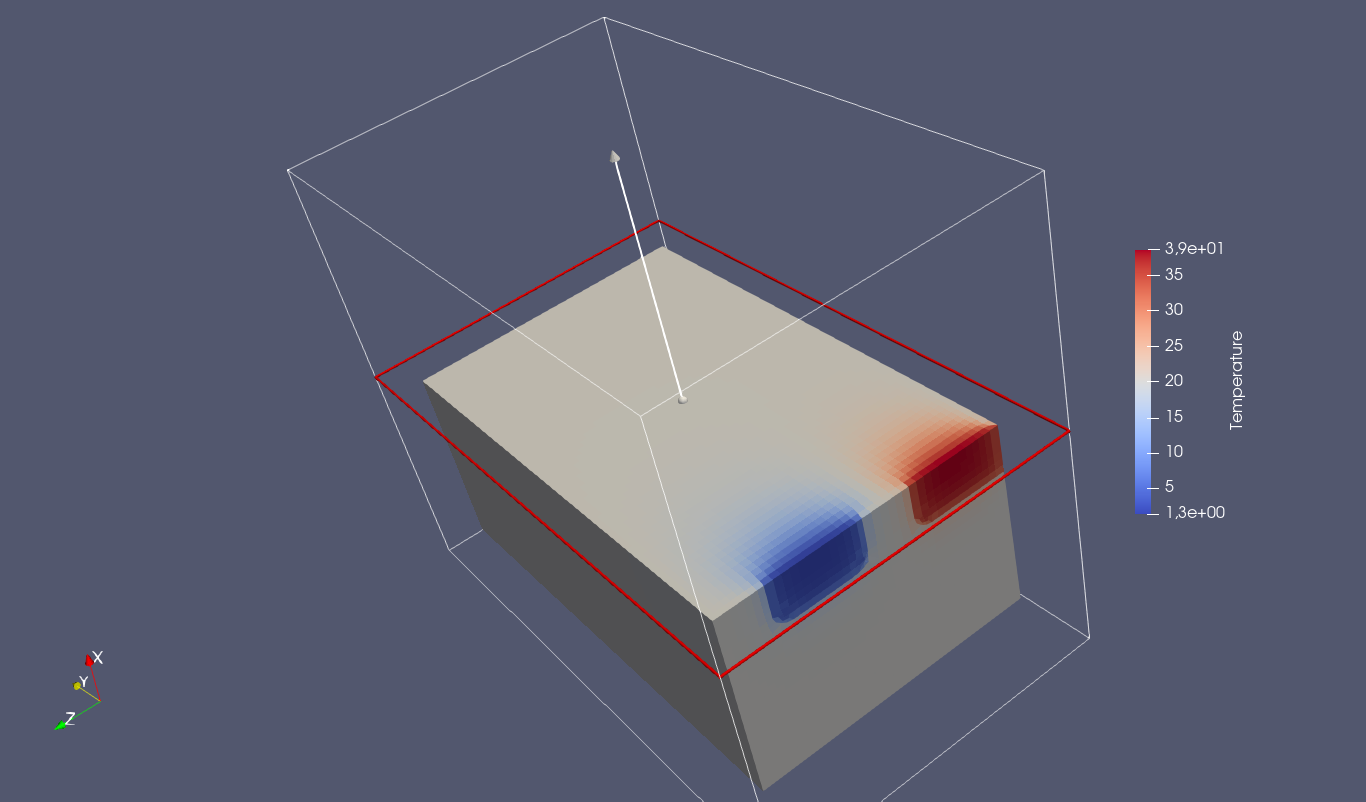
\includegraphics{Clipp.png} \textbar{}
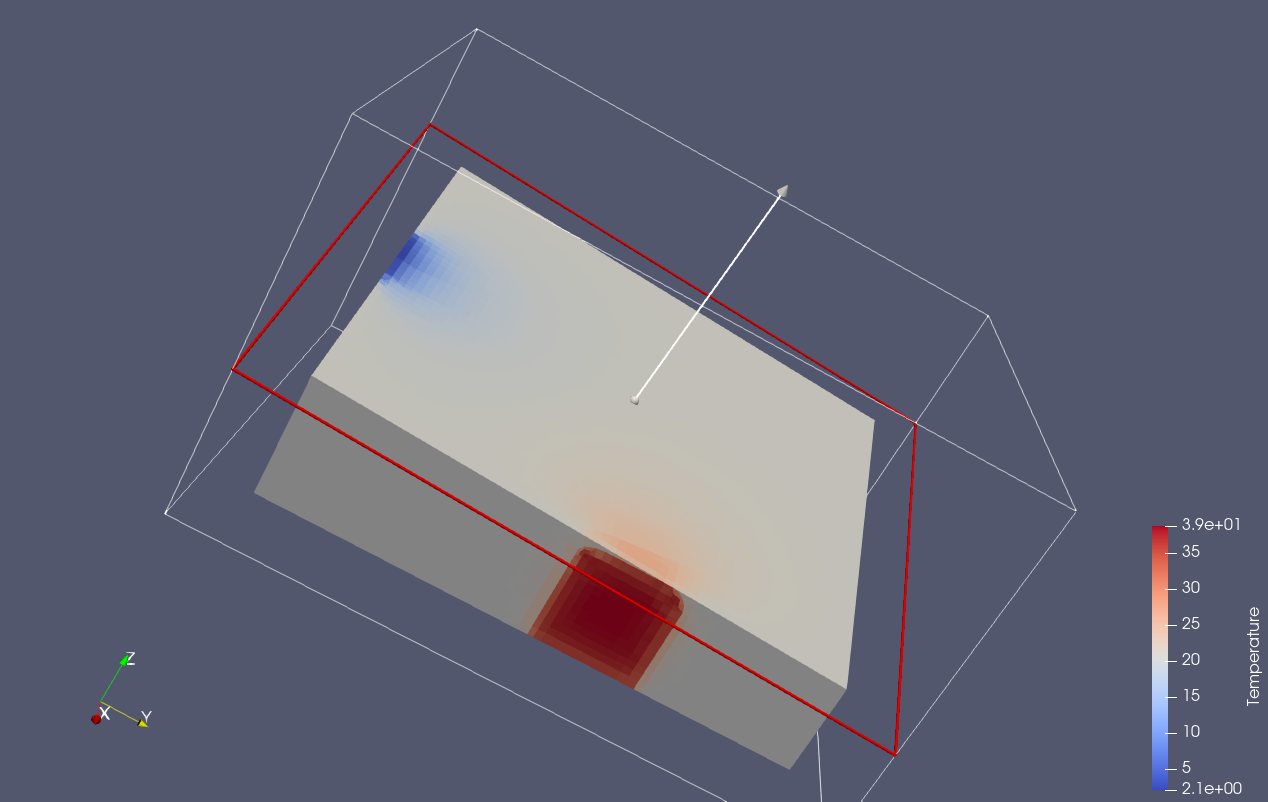
\includegraphics{ClipdroitCubic.png} \textbar{}
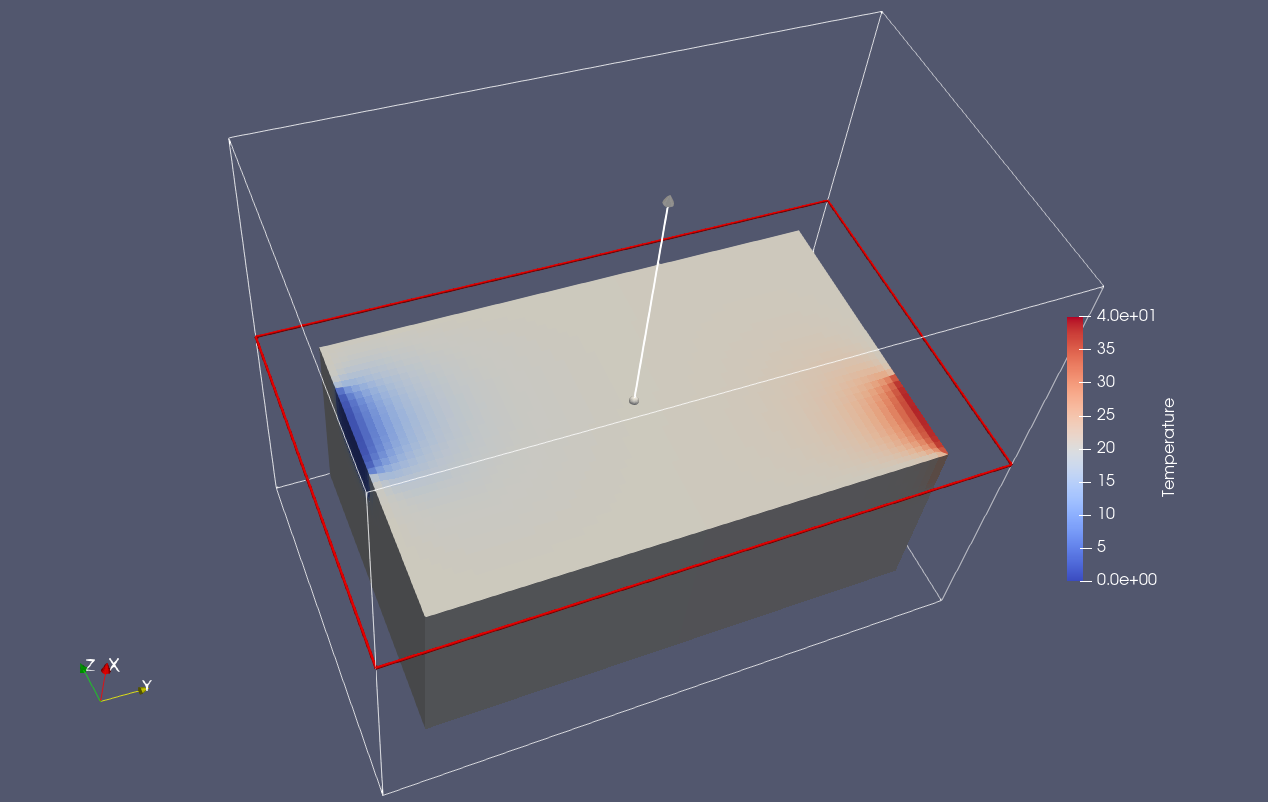
\includegraphics{ClippDevantCubs.png}

~ ~The volume of the cells for the temperature between \(18^\circ C\)
and \(22^\circ\) usint the integrate veriable function of Paraview are
given below.

\hypertarget{for-tetrahedral-we-have}{%
\paragraph{For tetrahedral we have:}\label{for-tetrahedral-we-have}}

Radiator under window\textbar{} Radiator on the right wall \textbar{}
Radiator in the wall in front of the window - \textbar{} - -\textbar{}-
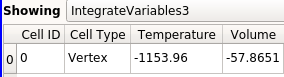
\includegraphics{IntearVar147655.png} \textbar{}
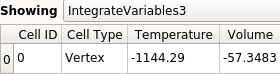
\includegraphics{IntVarDroitTetra.png} \textbar{}
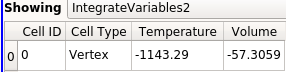
\includegraphics{IntVarDevanTetra.png}

~ ~From these results, we conclude that the best position for the
radiator is when it is place under the windows.

\hypertarget{for-cubic-mesh-we-have}{%
\paragraph{For cubic mesh we have:}\label{for-cubic-mesh-we-have}}

Radiator under window\textbar{} Radiator on the right wall \textbar{}
Radiator in the wall in front of the window - \textbar{} - -\textbar{}-
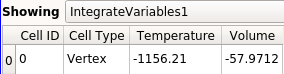
\includegraphics{IntegrateVariabl.png} \textbar{}
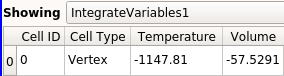
\includegraphics{IntVarDroitCubs.png} \textbar{}
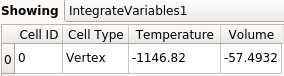
\includegraphics{IntVarDevantCubs.png}

~ ~We observe the same conclusion here.

    \hypertarget{comparison-between-result-with-cubes-and-tetrahedra}{%
\subsubsection{3.4 - Comparison between result with Cubes and
Tetrahedra}\label{comparison-between-result-with-cubes-and-tetrahedra}}

To compare the results obtained using the two meshes, we first consider
the case were the radiator is below the window. Using the paraview
Threshold operation followed by the paraview Integrate over variable
operation, we obtain the following results:

\begin{longtable}[]{@{}ll@{}}
\toprule
Tetrahedral mesh & Cubic mesh\tabularnewline
\midrule
\endhead
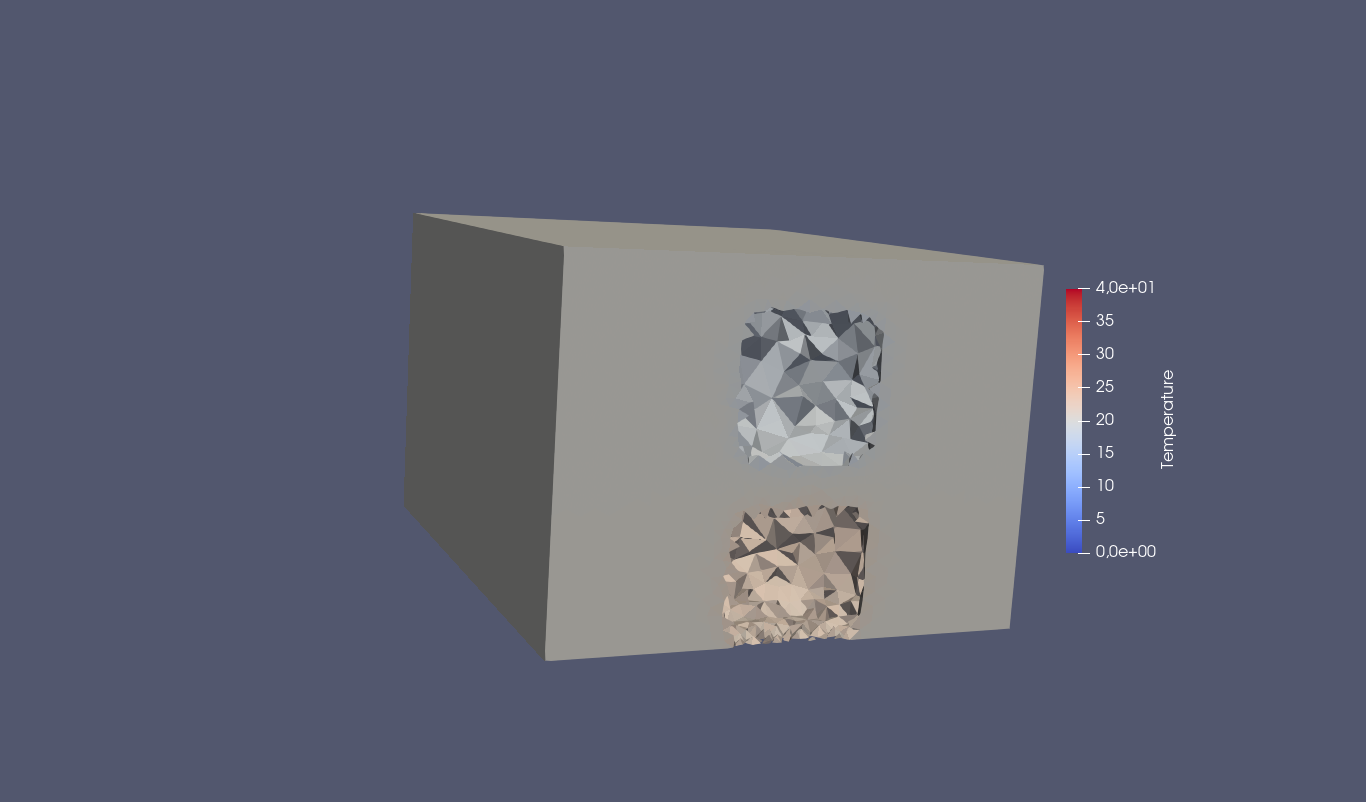
\includegraphics{TreshFVtetra147655.png} &
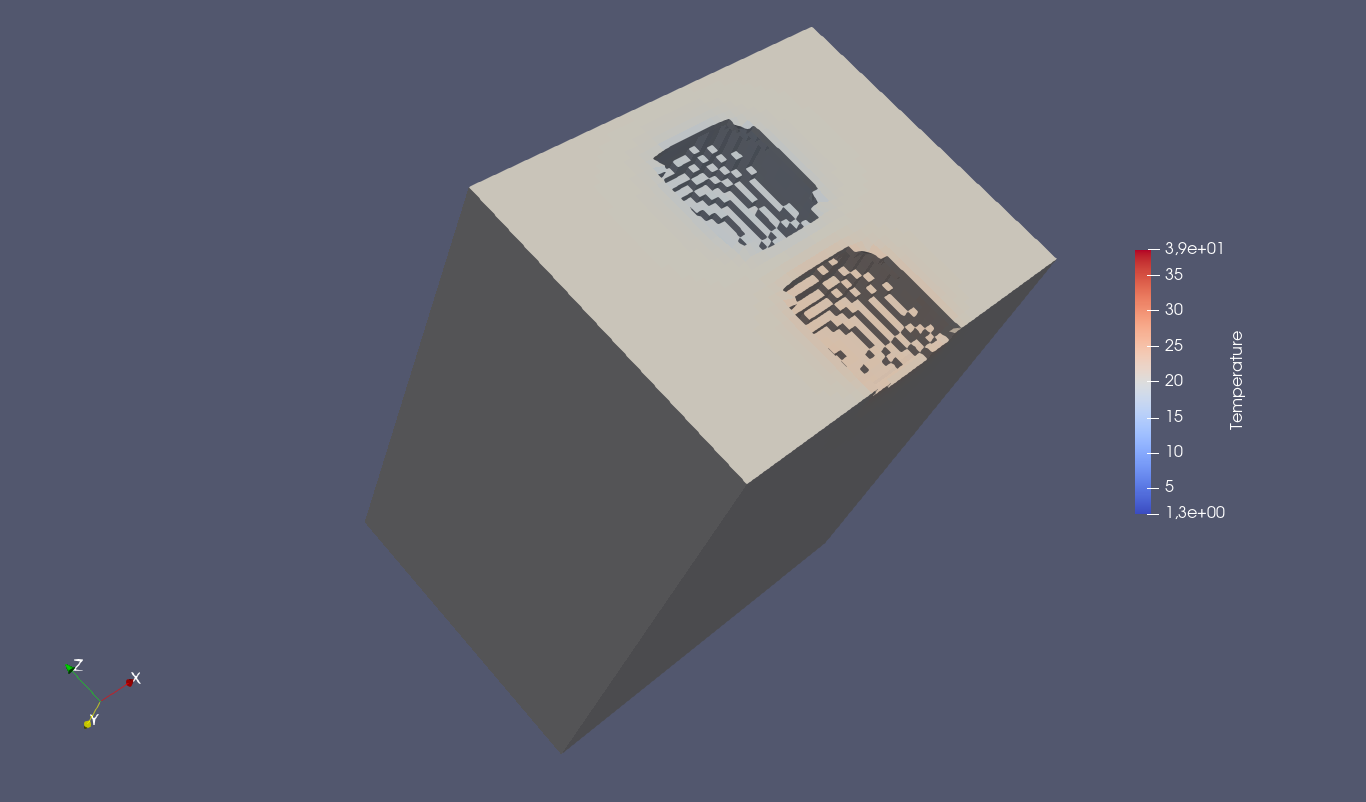
\includegraphics{Treshold140745.png}\tabularnewline
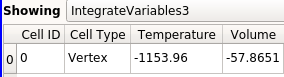
\includegraphics{IntearVar147655.png} &
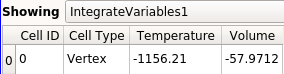
\includegraphics{IntegrateVariabl.png}\tabularnewline
\bottomrule
\end{longtable}

\#\#\#\# Conclusion

Taking the control volume of the two results, we observe that with the
cubic mesh we have 57.9712 which is greater than 57.8651 obtain in the
case of tretrahedral mesh even though the number of tetrahedrons is more
than the cubes. Hence, finite volume approximation gives better results
when using cubic mesh in 3D than tetrahedral mesh.

    \hypertarget{python-script}{%
\subsection{4 - Python script}\label{python-script}}

\begin{Shaded}
\begin{Highlighting}[]
\CommentTok{# -*-coding:utf-8 -*}
\CommentTok{#=======================================================================================================================}
\CommentTok{# Name        : Résolution VF de l'équation de Laplace 3D -\textbackslash{}Delta T = 0 avec conditions aux limites de Dirichlet u non nulle (fenetre et radiateur)}
\CommentTok{# Authors     : Michaël Ndjinga, Sédrick Kameni Ngwamou}
\CommentTok{# Copyright   : CEA Saclay 2019}
\CommentTok{# Description : Utilisation de la méthode des volumes finis avec champs u discrétisés aux cellules d'un maillage de cubes}
\CommentTok{#               Conditions limites correspondant au refroidissement dû à une fenêtre et au chauffage dû à un radiateur}
\CommentTok{#               Création et sauvegarde du champ résultant ainsi que du champ second membre en utilisant la librairie CDMATH}
\CommentTok{#=======================================================================================================================}

\ImportTok{import}\NormalTok{ CoreFlows }\ImportTok{as}\NormalTok{ cf}
\ImportTok{import}\NormalTok{ cdmath}
\ImportTok{import}\NormalTok{ PV_routines}
\ImportTok{import}\NormalTok{ VTK_routines}

\KeywordTok{def}\NormalTok{ StationaryDiffusionEquation_3DVF_RoomCooling(resolution):}
\NormalTok{    spaceDim }\OperatorTok{=} \DecValTok{3}\OperatorTok{;}
    
    \CommentTok{#Chargement du maillage cartésien du domaine}
    \CommentTok{#==============================================}
\NormalTok{    my_mesh }\OperatorTok{=}\NormalTok{ cdmath.Mesh(}\StringTok{'RoomCoulingCubeBon.med'}\NormalTok{)}\CommentTok{#Rom_CoulingCube2.med}
    
\NormalTok{    nbCells }\OperatorTok{=}\NormalTok{ my_mesh.getNumberOfCells()}
    \BuiltInTok{print} \StringTok{"Loaded Structured 3D mesh"}
    
    \CommentTok{#Conditions limites}
\NormalTok{    Tmur}\OperatorTok{=}\DecValTok{20}
\NormalTok{    Tfenetre}\OperatorTok{=}\DecValTok{0}
\NormalTok{    Tradiateur}\OperatorTok{=}\DecValTok{40}

\NormalTok{    FEComputation}\OperatorTok{=}\VariableTok{False}
\NormalTok{    myProblem }\OperatorTok{=}\NormalTok{ cf.StationaryDiffusionEquation(spaceDim,FEComputation)}\OperatorTok{;}
\NormalTok{    myProblem.setMesh(my_mesh)}\OperatorTok{;}
    
\NormalTok{    myProblem.setDirichletBoundaryCondition(}\StringTok{"Fenetre"}\NormalTok{,Tfenetre)}
\NormalTok{    myProblem.setDirichletBoundaryCondition(}\StringTok{"Radiateur_Dessous"}\NormalTok{,Tradiateur)}
\NormalTok{    myProblem.setDirichletBoundaryCondition(}\StringTok{"Radiateur_Devant"}\NormalTok{,Tmur)}
\NormalTok{    myProblem.setDirichletBoundaryCondition(}\StringTok{"Radiateur_Droit"}\NormalTok{,Tmur)}
\NormalTok{    myProblem.setDirichletBoundaryCondition(}\StringTok{"Murs"}\NormalTok{,Tmur)}

    \CommentTok{# name of result file}
\NormalTok{    fileName }\OperatorTok{=} \StringTok{"3DVF_StructuredCubes"}\OperatorTok{+}\BuiltInTok{str}\NormalTok{(nbCells)}\OperatorTok{;}

    \CommentTok{# computation parameters}
\NormalTok{    myProblem.setFileName(fileName)}\OperatorTok{;}

    \CommentTok{# Run the computation}
\NormalTok{    myProblem.initialize()}\OperatorTok{;}
    \BuiltInTok{print}\NormalTok{(}\StringTok{"Running python "}\OperatorTok{+}\NormalTok{ fileName )}\OperatorTok{;}

\NormalTok{    ok }\OperatorTok{=}\NormalTok{ myProblem.solveStationaryProblem()}\OperatorTok{;}
    \ControlFlowTok{if}\NormalTok{ (}\KeywordTok{not}\NormalTok{ ok):}
        \BuiltInTok{print}\NormalTok{( }\StringTok{"Python simulation of "} \OperatorTok{+}\NormalTok{ fileName }\OperatorTok{+} \StringTok{"  failed ! "}\NormalTok{ )}\OperatorTok{;}
        \ControlFlowTok{pass}
    \ControlFlowTok{else}\NormalTok{:}
        \BuiltInTok{print}\NormalTok{( }\StringTok{"Python simulation of "} \OperatorTok{+}\NormalTok{ fileName }\OperatorTok{+} \StringTok{"  successful ! "}\NormalTok{ )}\OperatorTok{;}
        \ControlFlowTok{pass}

\NormalTok{    myProblem.terminate()}\OperatorTok{;}
    
    \CommentTok{# save 2D picture}
\NormalTok{    VTK_routines.Clip_VTK_data_to_VTK(}\StringTok{"StationaryDiffusionEquation_3DVF_StructuredCubes"}\OperatorTok{+}\BuiltInTok{str}\NormalTok{(nbCells)}\OperatorTok{+}\StringTok{'_0.vtu'}\NormalTok{,}\StringTok{"Clip_VTK_data_to_VTK_"}\OperatorTok{+} \StringTok{"StationaryDiffusionEquation_3DVF_StructuredCubes_"}\OperatorTok{+}\BuiltInTok{str}\NormalTok{(nbCells)}\OperatorTok{+}\StringTok{'_0.vtu'}\NormalTok{,[}\FloatTok{0.5}\NormalTok{,}\FloatTok{0.5}\NormalTok{,}\FloatTok{0.5}\NormalTok{], [}\OperatorTok{-}\FloatTok{0.5}\NormalTok{,}\OperatorTok{-}\FloatTok{0.5}\NormalTok{,}\OperatorTok{-}\FloatTok{0.5}\NormalTok{],resolution )}
\NormalTok{    PV_routines.Save_PV_data_to_picture_file(}\StringTok{"Clip_VTK_data_to_VTK_"}\OperatorTok{+}\StringTok{"StationaryDiffusionEquation_3DVF_StructuredCubes_"}\OperatorTok{+}\BuiltInTok{str}\NormalTok{(nbCells)}\OperatorTok{+}\StringTok{'_0.vtu'}\NormalTok{,}\StringTok{"Temperature"}\NormalTok{,}\StringTok{'NODES'}\NormalTok{,}\StringTok{"Clip_VTK_data_to_VTK_"}\OperatorTok{+}\StringTok{"StationaryDiffusionEquation_3DVF_StructuredCubes_"}\OperatorTok{+}\BuiltInTok{str}\NormalTok{(nbCells))}
    \ControlFlowTok{return}\NormalTok{ ok}

\ControlFlowTok{if} \VariableTok{__name__} \OperatorTok{==} \StringTok{"""__main__"""}\NormalTok{:}
\NormalTok{    StationaryDiffusionEquation_3DVF_RoomCooling(}\DecValTok{100}\NormalTok{)}
    
    
\end{Highlighting}
\end{Shaded}

    \hypertarget{bibliography}{%
\subsection{5 - Bibliography}\label{bibliography}}

{[}1{]} Grégoire Allaire, Numerical analysis and optimization, Oxford
University Press, 2007

{[}2{]} R. Eymard, T. Gallouët, R. Herbin, Finite Volume Methods,
Handbook for Numerical Analysis, Ph. Ciarlet, J.L. Lions eds, North
Holland, 2000, 715-1022.


    % Add a bibliography block to the postdoc
    
    
    
    \end{document}
